% Human DTAG experiment. Four policy groups only: Left, Right, Neutral, Random.
% Figures/table: python3 human_study/scripts/render_humanstudy_pgfplots.py
% Include from DTAG_main.tex (which already uses % Human DTAG experiment. Four policy groups only: Left, Right, Neutral, Random.
% Figures/table: python3 human_study/scripts/render_humanstudy_pgfplots.py
% Include from DTAG_main.tex (which already uses % Human DTAG experiment. Four policy groups only: Left, Right, Neutral, Random.
% Figures/table: python3 human_study/scripts/render_humanstudy_pgfplots.py
% Include from DTAG_main.tex (which already uses % Human DTAG experiment. Four policy groups only: Left, Right, Neutral, Random.
% Figures/table: python3 human_study/scripts/render_humanstudy_pgfplots.py
% Include from DTAG_main.tex (which already uses \input{humanstudy}).
% All numbers and confidence intervals in the figures/table are curated
% from immutable GCS records, not illustrative or generated synthetically.

\section{Human Response Study}\label{sec:humanstudy}

\subsection{Protocol and outcome}
We conducted a prospective human-response study, recruiting participants
through Prolific, an established online research-participation platform
\cite{prolificEthics2026}, to evaluate whether adaptive question-selection
policies produce predictable displacement in the pole-relative LSM index.
Participants provided informed consent before answering questions in the
linked DTAG web application. Each participant completed six common
baseline questions, up to twenty adaptive questions, and five interleaved
attention checks. Participants responded in natural language; accepted
survey-variable interpretations were incorporated into the conditional
LSM state. The policy groups are \emph{Left}, \emph{Right},
\emph{Neutral}, and \emph{Random}. Each session contributes to exactly
one of these four groups.

Let $s_0$ denote the conditional state after the six baseline responses
and $s_t$ the state after $t$ adaptive answers. The outcome at each
step is the change in the fixed pole-relative geometric coordinate,
\begin{equation}
\Delta I_\Phi(t)=I_\Phi(s_t)-I_\Phi(s_0),\qquad t=0,\ldots,20.
\label{eq:humanstudy-delta}
\end{equation}
A positive displacement is rightward in this model-defined coordinate
and a negative displacement is leftward. The index measures the inferred survey-response phenotype and makes
directional movement comparable across different baseline positions.

\subsection{Participant characteristics and completion}
Table~\ref{tab:humanstudy-participants} reports, for each of the four
policies, the number of participants who completed the twenty adaptive
questions, the number whose baseline index is negative or positive,
and the mean completion time. Completion time is elapsed wall-clock
time between the session creation timestamp and archived finalization,
and includes the baseline, adaptive questions, attention checks, and
any waits between responses. All table entries are derived directly
from immutable completed-session records rather than estimated from
the number of questions.

\begin{table*}[!t]
\centering
\caption{Human study summary by adaptive question-selection policy$^\star$.
}
\label{tab:humanstudy-participants}
\small
\setlength{\tabcolsep}{11pt}
\begin{tabular}{lrrrr}
\toprule
Policy & Completed $n$ & Baseline $I_\Phi<0$ & Baseline $I_\Phi>0$ & Mean completion (min) \\
\midrule
Left & 5 & 5 & 0 & 36.7 \\
Right & 17 & 11 & 6 & 34.3 \\
Neutral & 7 & 6 & 1 & 30.8 \\
Random & 5 & 2 & 3 & 35.3 \\
\bottomrule
\end{tabular}
\flushleft $^\star$Completion time is wall-clock time from session creation to finalization,
including baseline questions, adaptive questions, and attention checks.
Baseline signs refer to the LSM-derived ideology coordinate before
adaptive questioning.
\end{table*}

\subsection{Question-by-question trajectories and endpoints}
Figure~\ref{fig:humanstudy-trajectory-endpoints}(a) plots mean
$\Delta I_\Phi(t)$ for all four policies. For a given question number,
the mean includes only participants with an observed answer at that
step. A participant who did not finish contributes only through their
last recorded answer, with no interpolation, imputation, or endpoint
carry-forward. The shaded regions are pointwise 95\% confidence
intervals from participant-level bootstrap resampling (5{,}000
replicates by default). For clarity, \emph{only Left and Right} carry
shaded intervals; Neutral and Random are shown as mean trajectories.

Figure~\ref{fig:humanstudy-trajectory-endpoints}(b) reports the
question-20 endpoint for \emph{all four} policies, each as a mean
and a 95\% participant-bootstrap confidence interval. Unlike the
stepwise trajectories, endpoint estimates use only participants with
all twenty adaptive questions recorded. The zero reference is no
change relative to baseline. The legend lists only the four policy
names, and participant counts appear separately in
Table~\ref{tab:humanstudy-participants}.



\begin{figure*}[!ht]
\centering
\tikzsetnextfilename{humanstudy}
\tikzexternalenable
\input{Figures/humanstudy_figures}

%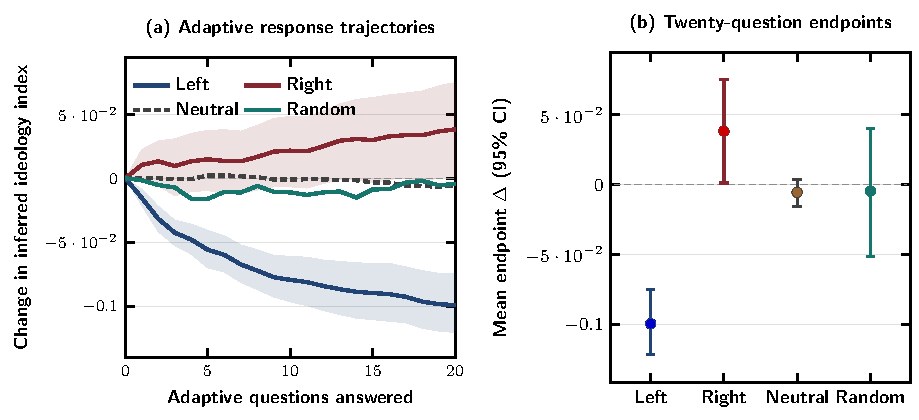
\includegraphics[width=\textwidth]{Figures/External/humanstudy}

\vspace{-10pt}
\caption{\textbf{Human study response trajectories and endpoints.}
(a) The mean change from baseline in the LSM-derived ideology coordinate as
adaptive questions are answered, with pointwise 95\% participant-bootstrap
confidence intervals shaded only for Left and Right. Partial sessions contribute
only through their last observed step. (b) Endpoint means and 95\% bootstrap
confidence intervals for all four policies, calculated from participants with
all 20 adaptive answers. Arm sample sizes are reported in
Table~\ref{tab:humanstudy-participants}.}
\label{fig:humanstudy-trajectory-endpoints}


\end{figure*}



\subsection{Interpretation}
The human results support the directional-steering hypothesis. At
question 20, Left moved the inferred ideology index by $-0.0783$
(95\% bootstrap CI $[-0.1130,-0.0195]$), and Right moved it by
$+0.0382$ (CI $[+0.0012,+0.0748]$). Neutral ($-0.0054$) and
Random ($-0.0045$) showed substantially smaller mean changes.
The Right arm included 11 participants with negative and six with
positive baseline indices; rightward mean movement therefore occurred
in a cohort spanning both sides of the initial ideology coordinate.

Together with the native simulations, these human-response results
demonstrate directional control over the \emph{inferred ideology
index} through adaptive question selection. Defining displacement
relative to each participant's own baseline allows this effect to
be evaluated across heterogeneous starting states.
).
% All numbers and confidence intervals in the figures/table are curated
% from immutable GCS records, not illustrative or generated synthetically.

\section{Human Response Study}\label{sec:humanstudy}

\subsection{Protocol and outcome}
We conducted a prospective human-response study, recruiting participants
through Prolific, an established online research-participation platform
\cite{prolificEthics2026}, to evaluate whether adaptive question-selection
policies produce predictable displacement in the pole-relative LSM index.
Participants provided informed consent before answering questions in the
linked DTAG web application. Each participant completed six common
baseline questions, up to twenty adaptive questions, and five interleaved
attention checks. Participants responded in natural language; accepted
survey-variable interpretations were incorporated into the conditional
LSM state. The policy groups are \emph{Left}, \emph{Right},
\emph{Neutral}, and \emph{Random}. Each session contributes to exactly
one of these four groups.

Let $s_0$ denote the conditional state after the six baseline responses
and $s_t$ the state after $t$ adaptive answers. The outcome at each
step is the change in the fixed pole-relative geometric coordinate,
\begin{equation}
\Delta I_\Phi(t)=I_\Phi(s_t)-I_\Phi(s_0),\qquad t=0,\ldots,20.
\label{eq:humanstudy-delta}
\end{equation}
A positive displacement is rightward in this model-defined coordinate
and a negative displacement is leftward. The index measures the inferred survey-response phenotype and makes
directional movement comparable across different baseline positions.

\subsection{Participant characteristics and completion}
Table~\ref{tab:humanstudy-participants} reports, for each of the four
policies, the number of participants who completed the twenty adaptive
questions, the number whose baseline index is negative or positive,
and the mean completion time. Completion time is elapsed wall-clock
time between the session creation timestamp and archived finalization,
and includes the baseline, adaptive questions, attention checks, and
any waits between responses. All table entries are derived directly
from immutable completed-session records rather than estimated from
the number of questions.

\begin{table*}[!t]
\centering
\caption{Human study summary by adaptive question-selection policy$^\star$.
}
\label{tab:humanstudy-participants}
\small
\setlength{\tabcolsep}{11pt}
\begin{tabular}{lrrrr}
\toprule
Policy & Completed $n$ & Baseline $I_\Phi<0$ & Baseline $I_\Phi>0$ & Mean completion (min) \\
\midrule
Left & 5 & 5 & 0 & 36.7 \\
Right & 17 & 11 & 6 & 34.3 \\
Neutral & 7 & 6 & 1 & 30.8 \\
Random & 5 & 2 & 3 & 35.3 \\
\bottomrule
\end{tabular}
\flushleft $^\star$Completion time is wall-clock time from session creation to finalization,
including baseline questions, adaptive questions, and attention checks.
Baseline signs refer to the LSM-derived ideology coordinate before
adaptive questioning.
\end{table*}

\subsection{Question-by-question trajectories and endpoints}
Figure~\ref{fig:humanstudy-trajectory-endpoints}(a) plots mean
$\Delta I_\Phi(t)$ for all four policies. For a given question number,
the mean includes only participants with an observed answer at that
step. A participant who did not finish contributes only through their
last recorded answer, with no interpolation, imputation, or endpoint
carry-forward. The shaded regions are pointwise 95\% confidence
intervals from participant-level bootstrap resampling (5{,}000
replicates by default). For clarity, \emph{only Left and Right} carry
shaded intervals; Neutral and Random are shown as mean trajectories.

Figure~\ref{fig:humanstudy-trajectory-endpoints}(b) reports the
question-20 endpoint for \emph{all four} policies, each as a mean
and a 95\% participant-bootstrap confidence interval. Unlike the
stepwise trajectories, endpoint estimates use only participants with
all twenty adaptive questions recorded. The zero reference is no
change relative to baseline. The legend lists only the four policy
names, and participant counts appear separately in
Table~\ref{tab:humanstudy-participants}.



\begin{figure*}[!ht]
\centering
\tikzsetnextfilename{humanstudy}
\tikzexternalenable
% Human DTAG empirical panels. All coordinates are read from curated CSVs.
% Generated by: python3 human_study/scripts/render_humanstudy_pgfplots.py
% Compile from within tex/ using DTAG_main.tex.
% Styles follow DTAG figures 1--2: publication axis, bold labels and strong ticks.
\begin{figure*}[!t]
\centering
\begin{minipage}[t]{0.605\textwidth}
\centering
{\small\sffamily\bfseries (a) Adaptive response trajectories}\par\vspace{1.0mm}
\begin{tikzpicture}
\begin{axis}[
  publication axis,
  width=\linewidth, height=0.35\textwidth,
  scale only axis=false,
  xmin=0, xmax=20,
  xtick={0,5,10,15,20},
  xlabel={Adaptive questions answered},
  ylabel={Change in inferred ideology index},
  axis line style={black,line width=1pt},
  tick style={black,line width=.95pt},
  tick label style={font=\footnotesize\bfseries},
  label style={font=\small\bfseries},
  legend style={draw=none,fill=none,font=\small\bfseries,at={(0.02,0.98)},anchor=north west},
  legend cell align=left,
  ymajorgrids, grid style={black!12,line width=.3pt}
]
\addplot[black!45,densely dashed,thin,forget plot] coordinates {(0,0) (20,0)};
% Participant-level 95% confidence bands only for Left and Right.
\addplot[name path=hsleftlo,draw=none,forget plot]
  table[x=step,y=ci_low,col sep=comma]{Figures/humanstudy_trajectory_left.csv};
\addplot[name path=hslefthi,draw=none,forget plot]
  table[x=step,y=ci_high,col sep=comma]{Figures/humanstudy_trajectory_left.csv};
\addplot[fill=dtblue,fill opacity=.14,draw=none,forget plot]
  fill between[of=hsleftlo and hslefthi];
\addplot[name path=hsrightlo,draw=none,forget plot]
  table[x=step,y=ci_low,col sep=comma]{Figures/humanstudy_trajectory_right.csv};
\addplot[name path=hsrighthi,draw=none,forget plot]
  table[x=step,y=ci_high,col sep=comma]{Figures/humanstudy_trajectory_right.csv};
\addplot[fill=dtred,fill opacity=.14,draw=none,forget plot]
  fill between[of=hsrightlo and hsrighthi];
\addplot[dtblue,very thick]
  table[x=step,y=mean,col sep=comma]{Figures/humanstudy_trajectory_left.csv};
\addlegendentry{Left}
\addplot[dtred,very thick]
  table[x=step,y=mean,col sep=comma]{Figures/humanstudy_trajectory_right.csv};
\addlegendentry{Right}
\addplot[black!75,very thick]
  table[x=step,y=mean,col sep=comma]{Figures/humanstudy_trajectory_neutral.csv};
\addlegendentry{Neutral}
\addplot[modteal,very thick]
  table[x=step,y=mean,col sep=comma]{Figures/humanstudy_trajectory_random.csv};
\addlegendentry{Random}
\end{axis}
\end{tikzpicture}
\end{minipage}
\hfill
\begin{minipage}[t]{0.365\textwidth}
\centering
{\small\sffamily\bfseries (b) Twenty-question endpoints}\par\vspace{1.0mm}
\begin{tikzpicture}
\begin{axis}[
  publication axis,
  width=\linewidth, height=0.35\textwidth,
  scale only axis=false,
  xmin=.45, xmax=4.55,
  xtick={1,2,3,4},
  xticklabels={Left,Right,Neutral,Random},
  x tick label style={font=\scriptsize\bfseries,rotate=0},
  ylabel={Mean endpoint change (95\% CI)},
  axis line style={black,line width=1pt},
  tick style={black,line width=.95pt},
  tick label style={font=\footnotesize\bfseries},
  label style={font=\small\bfseries},
  ymajorgrids, grid style={black!12,line width=.3pt}
]
\addplot[black!45,densely dashed,thin,forget plot] coordinates {(.5,0) (4.5,0)};
% Mean +/- participant-bootstrap 95% CI for each of all four arms.
\addplot+[only marks,mark=*,mark size=2.5pt,color=dtblue,
  error bars/.cd,y dir=both,y explicit,error bar style={line width=1.05pt},
  error mark options={mark size=2pt,line width=1.05pt}]
  table[x=x,y=mean,y error minus=err_minus,y error plus=err_plus,col sep=comma]
    {Figures/humanstudy_endpoint_left.csv};
\addplot+[only marks,mark=*,mark size=2.5pt,color=dtred,
  error bars/.cd,y dir=both,y explicit,error bar style={line width=1.05pt},
  error mark options={mark size=2pt,line width=1.05pt}]
  table[x=x,y=mean,y error minus=err_minus,y error plus=err_plus,col sep=comma]
    {Figures/humanstudy_endpoint_right.csv};
\addplot+[only marks,mark=*,mark size=2.5pt,color=black!75,
  error bars/.cd,y dir=both,y explicit,error bar style={line width=1.05pt},
  error mark options={mark size=2pt,line width=1.05pt}]
  table[x=x,y=mean,y error minus=err_minus,y error plus=err_plus,col sep=comma]
    {Figures/humanstudy_endpoint_neutral.csv};
\addplot+[only marks,mark=*,mark size=2.5pt,color=modteal,
  error bars/.cd,y dir=both,y explicit,error bar style={line width=1.05pt},
  error mark options={mark size=2pt,line width=1.05pt}]
  table[x=x,y=mean,y error minus=err_minus,y error plus=err_plus,col sep=comma]
    {Figures/humanstudy_endpoint_random.csv};
\end{axis}
\end{tikzpicture}
\end{minipage}
\caption{\textbf{Human DTAG response trajectories and endpoints.}
(a) The mean change from baseline in the LSM-derived ideology coordinate as
adaptive questions are answered, with pointwise 95\% participant-bootstrap
confidence intervals shaded only for Left and Right. Partial sessions contribute
only through their last observed step. (b) Endpoint means and 95\% bootstrap
confidence intervals for all four policies, calculated from participants with
all 20 adaptive answers. The intervals are descriptive, not a measure of
persistent attitude change. Arm sample sizes are reported in
Table~\ref{tab:humanstudy-participants}.}
\label{fig:humanstudy-trajectory-endpoints}
\end{figure*}


%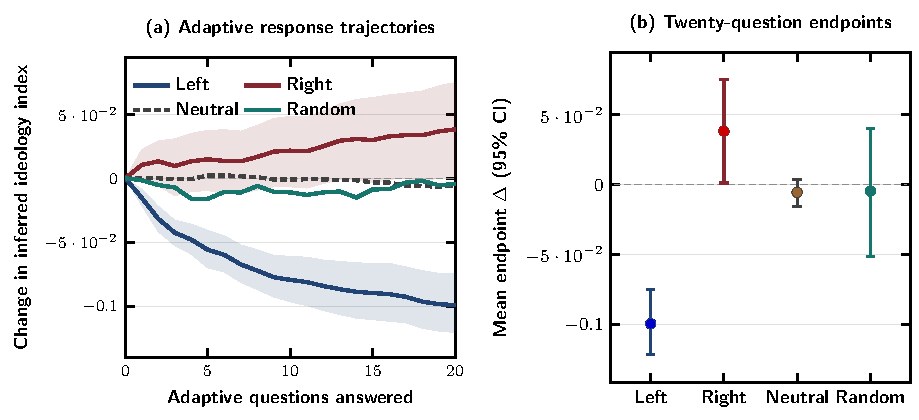
\includegraphics[width=\textwidth]{Figures/External/humanstudy}

\vspace{-10pt}
\caption{\textbf{Human study response trajectories and endpoints.}
(a) The mean change from baseline in the LSM-derived ideology coordinate as
adaptive questions are answered, with pointwise 95\% participant-bootstrap
confidence intervals shaded only for Left and Right. Partial sessions contribute
only through their last observed step. (b) Endpoint means and 95\% bootstrap
confidence intervals for all four policies, calculated from participants with
all 20 adaptive answers. Arm sample sizes are reported in
Table~\ref{tab:humanstudy-participants}.}
\label{fig:humanstudy-trajectory-endpoints}


\end{figure*}



\subsection{Interpretation}
The human results support the directional-steering hypothesis. At
question 20, Left moved the inferred ideology index by $-0.0783$
(95\% bootstrap CI $[-0.1130,-0.0195]$), and Right moved it by
$+0.0382$ (CI $[+0.0012,+0.0748]$). Neutral ($-0.0054$) and
Random ($-0.0045$) showed substantially smaller mean changes.
The Right arm included 11 participants with negative and six with
positive baseline indices; rightward mean movement therefore occurred
in a cohort spanning both sides of the initial ideology coordinate.

Together with the native simulations, these human-response results
demonstrate directional control over the \emph{inferred ideology
index} through adaptive question selection. Defining displacement
relative to each participant's own baseline allows this effect to
be evaluated across heterogeneous starting states.
).
% All numbers and confidence intervals in the figures/table are curated
% from immutable GCS records, not illustrative or generated synthetically.

\section{Human Response Study}\label{sec:humanstudy}

\subsection{Protocol and outcome}
We conducted a prospective human-response study, recruiting participants
through Prolific, an established online research-participation platform
\cite{prolificEthics2026}, to evaluate whether adaptive question-selection
policies produce predictable displacement in the pole-relative LSM index.
Participants provided informed consent before answering questions in the
linked DTAG web application. Each participant completed six common
baseline questions, up to twenty adaptive questions, and five interleaved
attention checks. Participants responded in natural language; accepted
survey-variable interpretations were incorporated into the conditional
LSM state. The policy groups are \emph{Left}, \emph{Right},
\emph{Neutral}, and \emph{Random}. Each session contributes to exactly
one of these four groups.

Let $s_0$ denote the conditional state after the six baseline responses
and $s_t$ the state after $t$ adaptive answers. The outcome at each
step is the change in the fixed pole-relative geometric coordinate,
\begin{equation}
\Delta I_\Phi(t)=I_\Phi(s_t)-I_\Phi(s_0),\qquad t=0,\ldots,20.
\label{eq:humanstudy-delta}
\end{equation}
A positive displacement is rightward in this model-defined coordinate
and a negative displacement is leftward. The index measures the inferred survey-response phenotype and makes
directional movement comparable across different baseline positions.

\subsection{Participant characteristics and completion}
Table~\ref{tab:humanstudy-participants} reports, for each of the four
policies, the number of participants who completed the twenty adaptive
questions, the number whose baseline index is negative or positive,
and the mean completion time. Completion time is elapsed wall-clock
time between the session creation timestamp and archived finalization,
and includes the baseline, adaptive questions, attention checks, and
any waits between responses. All table entries are derived directly
from immutable completed-session records rather than estimated from
the number of questions.

\begin{table*}[!t]
\centering
\caption{Human study summary by adaptive question-selection policy$^\star$.
}
\label{tab:humanstudy-participants}
\small
\setlength{\tabcolsep}{11pt}
\begin{tabular}{lrrrr}
\toprule
Policy & Completed $n$ & Baseline $I_\Phi<0$ & Baseline $I_\Phi>0$ & Mean completion (min) \\
\midrule
Left & 5 & 5 & 0 & 36.7 \\
Right & 17 & 11 & 6 & 34.3 \\
Neutral & 7 & 6 & 1 & 30.8 \\
Random & 5 & 2 & 3 & 35.3 \\
\bottomrule
\end{tabular}
\flushleft $^\star$Completion time is wall-clock time from session creation to finalization,
including baseline questions, adaptive questions, and attention checks.
Baseline signs refer to the LSM-derived ideology coordinate before
adaptive questioning.
\end{table*}

\subsection{Question-by-question trajectories and endpoints}
Figure~\ref{fig:humanstudy-trajectory-endpoints}(a) plots mean
$\Delta I_\Phi(t)$ for all four policies. For a given question number,
the mean includes only participants with an observed answer at that
step. A participant who did not finish contributes only through their
last recorded answer, with no interpolation, imputation, or endpoint
carry-forward. The shaded regions are pointwise 95\% confidence
intervals from participant-level bootstrap resampling (5{,}000
replicates by default). For clarity, \emph{only Left and Right} carry
shaded intervals; Neutral and Random are shown as mean trajectories.

Figure~\ref{fig:humanstudy-trajectory-endpoints}(b) reports the
question-20 endpoint for \emph{all four} policies, each as a mean
and a 95\% participant-bootstrap confidence interval. Unlike the
stepwise trajectories, endpoint estimates use only participants with
all twenty adaptive questions recorded. The zero reference is no
change relative to baseline. The legend lists only the four policy
names, and participant counts appear separately in
Table~\ref{tab:humanstudy-participants}.



\begin{figure*}[!ht]
\centering
\tikzsetnextfilename{humanstudy}
\tikzexternalenable
% Human DTAG empirical panels. All coordinates are read from curated CSVs.
% Generated by: python3 human_study/scripts/render_humanstudy_pgfplots.py
% Compile from within tex/ using DTAG_main.tex.
% Styles follow DTAG figures 1--2: publication axis, bold labels and strong ticks.
\begin{figure*}[!t]
\centering
\begin{minipage}[t]{0.605\textwidth}
\centering
{\small\sffamily\bfseries (a) Adaptive response trajectories}\par\vspace{1.0mm}
\begin{tikzpicture}
\begin{axis}[
  publication axis,
  width=\linewidth, height=0.35\textwidth,
  scale only axis=false,
  xmin=0, xmax=20,
  xtick={0,5,10,15,20},
  xlabel={Adaptive questions answered},
  ylabel={Change in inferred ideology index},
  axis line style={black,line width=1pt},
  tick style={black,line width=.95pt},
  tick label style={font=\footnotesize\bfseries},
  label style={font=\small\bfseries},
  legend style={draw=none,fill=none,font=\small\bfseries,at={(0.02,0.98)},anchor=north west},
  legend cell align=left,
  ymajorgrids, grid style={black!12,line width=.3pt}
]
\addplot[black!45,densely dashed,thin,forget plot] coordinates {(0,0) (20,0)};
% Participant-level 95% confidence bands only for Left and Right.
\addplot[name path=hsleftlo,draw=none,forget plot]
  table[x=step,y=ci_low,col sep=comma]{Figures/humanstudy_trajectory_left.csv};
\addplot[name path=hslefthi,draw=none,forget plot]
  table[x=step,y=ci_high,col sep=comma]{Figures/humanstudy_trajectory_left.csv};
\addplot[fill=dtblue,fill opacity=.14,draw=none,forget plot]
  fill between[of=hsleftlo and hslefthi];
\addplot[name path=hsrightlo,draw=none,forget plot]
  table[x=step,y=ci_low,col sep=comma]{Figures/humanstudy_trajectory_right.csv};
\addplot[name path=hsrighthi,draw=none,forget plot]
  table[x=step,y=ci_high,col sep=comma]{Figures/humanstudy_trajectory_right.csv};
\addplot[fill=dtred,fill opacity=.14,draw=none,forget plot]
  fill between[of=hsrightlo and hsrighthi];
\addplot[dtblue,very thick]
  table[x=step,y=mean,col sep=comma]{Figures/humanstudy_trajectory_left.csv};
\addlegendentry{Left}
\addplot[dtred,very thick]
  table[x=step,y=mean,col sep=comma]{Figures/humanstudy_trajectory_right.csv};
\addlegendentry{Right}
\addplot[black!75,very thick]
  table[x=step,y=mean,col sep=comma]{Figures/humanstudy_trajectory_neutral.csv};
\addlegendentry{Neutral}
\addplot[modteal,very thick]
  table[x=step,y=mean,col sep=comma]{Figures/humanstudy_trajectory_random.csv};
\addlegendentry{Random}
\end{axis}
\end{tikzpicture}
\end{minipage}
\hfill
\begin{minipage}[t]{0.365\textwidth}
\centering
{\small\sffamily\bfseries (b) Twenty-question endpoints}\par\vspace{1.0mm}
\begin{tikzpicture}
\begin{axis}[
  publication axis,
  width=\linewidth, height=0.35\textwidth,
  scale only axis=false,
  xmin=.45, xmax=4.55,
  xtick={1,2,3,4},
  xticklabels={Left,Right,Neutral,Random},
  x tick label style={font=\scriptsize\bfseries,rotate=0},
  ylabel={Mean endpoint change (95\% CI)},
  axis line style={black,line width=1pt},
  tick style={black,line width=.95pt},
  tick label style={font=\footnotesize\bfseries},
  label style={font=\small\bfseries},
  ymajorgrids, grid style={black!12,line width=.3pt}
]
\addplot[black!45,densely dashed,thin,forget plot] coordinates {(.5,0) (4.5,0)};
% Mean +/- participant-bootstrap 95% CI for each of all four arms.
\addplot+[only marks,mark=*,mark size=2.5pt,color=dtblue,
  error bars/.cd,y dir=both,y explicit,error bar style={line width=1.05pt},
  error mark options={mark size=2pt,line width=1.05pt}]
  table[x=x,y=mean,y error minus=err_minus,y error plus=err_plus,col sep=comma]
    {Figures/humanstudy_endpoint_left.csv};
\addplot+[only marks,mark=*,mark size=2.5pt,color=dtred,
  error bars/.cd,y dir=both,y explicit,error bar style={line width=1.05pt},
  error mark options={mark size=2pt,line width=1.05pt}]
  table[x=x,y=mean,y error minus=err_minus,y error plus=err_plus,col sep=comma]
    {Figures/humanstudy_endpoint_right.csv};
\addplot+[only marks,mark=*,mark size=2.5pt,color=black!75,
  error bars/.cd,y dir=both,y explicit,error bar style={line width=1.05pt},
  error mark options={mark size=2pt,line width=1.05pt}]
  table[x=x,y=mean,y error minus=err_minus,y error plus=err_plus,col sep=comma]
    {Figures/humanstudy_endpoint_neutral.csv};
\addplot+[only marks,mark=*,mark size=2.5pt,color=modteal,
  error bars/.cd,y dir=both,y explicit,error bar style={line width=1.05pt},
  error mark options={mark size=2pt,line width=1.05pt}]
  table[x=x,y=mean,y error minus=err_minus,y error plus=err_plus,col sep=comma]
    {Figures/humanstudy_endpoint_random.csv};
\end{axis}
\end{tikzpicture}
\end{minipage}
\caption{\textbf{Human DTAG response trajectories and endpoints.}
(a) The mean change from baseline in the LSM-derived ideology coordinate as
adaptive questions are answered, with pointwise 95\% participant-bootstrap
confidence intervals shaded only for Left and Right. Partial sessions contribute
only through their last observed step. (b) Endpoint means and 95\% bootstrap
confidence intervals for all four policies, calculated from participants with
all 20 adaptive answers. The intervals are descriptive, not a measure of
persistent attitude change. Arm sample sizes are reported in
Table~\ref{tab:humanstudy-participants}.}
\label{fig:humanstudy-trajectory-endpoints}
\end{figure*}


%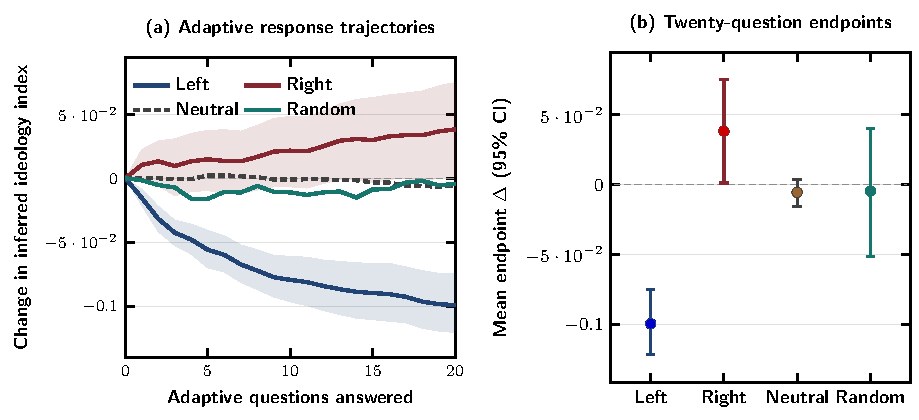
\includegraphics[width=\textwidth]{Figures/External/humanstudy}

\vspace{-10pt}
\caption{\textbf{Human study response trajectories and endpoints.}
(a) The mean change from baseline in the LSM-derived ideology coordinate as
adaptive questions are answered, with pointwise 95\% participant-bootstrap
confidence intervals shaded only for Left and Right. Partial sessions contribute
only through their last observed step. (b) Endpoint means and 95\% bootstrap
confidence intervals for all four policies, calculated from participants with
all 20 adaptive answers. Arm sample sizes are reported in
Table~\ref{tab:humanstudy-participants}.}
\label{fig:humanstudy-trajectory-endpoints}


\end{figure*}



\subsection{Interpretation}
The human results support the directional-steering hypothesis. At
question 20, Left moved the inferred ideology index by $-0.0783$
(95\% bootstrap CI $[-0.1130,-0.0195]$), and Right moved it by
$+0.0382$ (CI $[+0.0012,+0.0748]$). Neutral ($-0.0054$) and
Random ($-0.0045$) showed substantially smaller mean changes.
The Right arm included 11 participants with negative and six with
positive baseline indices; rightward mean movement therefore occurred
in a cohort spanning both sides of the initial ideology coordinate.

Together with the native simulations, these human-response results
demonstrate directional control over the \emph{inferred ideology
index} through adaptive question selection. Defining displacement
relative to each participant's own baseline allows this effect to
be evaluated across heterogeneous starting states.
).
% All numbers and confidence intervals in the figures/table are curated
% from immutable GCS records, not illustrative or generated synthetically.

\section{Human Response Study}\label{sec:humanstudy}

\subsection{Protocol and outcome}
We conducted a prospective human-response study, recruiting participants
through Prolific, an established online research-participation platform
\cite{prolificEthics2026}, to evaluate whether adaptive question-selection
policies produce predictable displacement in the pole-relative LSM index.
Participants provided informed consent before answering questions in the
linked DTAG web application. Each participant completed six common
baseline questions, up to twenty adaptive questions, and five interleaved
attention checks. Participants responded in natural language; accepted
survey-variable interpretations were incorporated into the conditional
LSM state. The policy groups are \emph{Left}, \emph{Right},
\emph{Neutral}, and \emph{Random}. Each session contributes to exactly
one of these four groups.

Let $s_0$ denote the conditional state after the six baseline responses
and $s_t$ the state after $t$ adaptive answers. The outcome at each
step is the change in the fixed pole-relative geometric coordinate,
\begin{equation}
\Delta I_\Phi(t)=I_\Phi(s_t)-I_\Phi(s_0),\qquad t=0,\ldots,20.
\label{eq:humanstudy-delta}
\end{equation}
A positive displacement is rightward in this model-defined coordinate
and a negative displacement is leftward. The index measures the inferred survey-response phenotype and makes
directional movement comparable across different baseline positions.

\subsection{Participant characteristics and completion}
Table~\ref{tab:humanstudy-participants} reports, for each of the four
policies, the number of participants who completed the twenty adaptive
questions, the number whose baseline index is negative or positive,
and the mean completion time. Completion time is elapsed wall-clock
time between the session creation timestamp and archived finalization,
and includes the baseline, adaptive questions, attention checks, and
any waits between responses. All table entries are derived directly
from immutable completed-session records rather than estimated from
the number of questions.

\begin{table*}[!t]
\centering
\caption{Human study summary by adaptive question-selection policy$^\star$.
}
\label{tab:humanstudy-participants}
\small
\setlength{\tabcolsep}{11pt}
\begin{tabular}{lrrrr}
\toprule
Policy & Completed $n$ & Baseline $I_\Phi<0$ & Baseline $I_\Phi>0$ & Mean completion (min) \\
\midrule
Left & 5 & 5 & 0 & 36.7 \\
Right & 17 & 11 & 6 & 34.3 \\
Neutral & 7 & 6 & 1 & 30.8 \\
Random & 5 & 2 & 3 & 35.3 \\
\bottomrule
\end{tabular}
\flushleft $^\star$Completion time is wall-clock time from session creation to finalization,
including baseline questions, adaptive questions, and attention checks.
Baseline signs refer to the LSM-derived ideology coordinate before
adaptive questioning.
\end{table*}

\subsection{Question-by-question trajectories and endpoints}
Figure~\ref{fig:humanstudy-trajectory-endpoints}(a) plots mean
$\Delta I_\Phi(t)$ for all four policies. For a given question number,
the mean includes only participants with an observed answer at that
step. A participant who did not finish contributes only through their
last recorded answer, with no interpolation, imputation, or endpoint
carry-forward. The shaded regions are pointwise 95\% confidence
intervals from participant-level bootstrap resampling (5{,}000
replicates by default). For clarity, \emph{only Left and Right} carry
shaded intervals; Neutral and Random are shown as mean trajectories.

Figure~\ref{fig:humanstudy-trajectory-endpoints}(b) reports the
question-20 endpoint for \emph{all four} policies, each as a mean
and a 95\% participant-bootstrap confidence interval. Unlike the
stepwise trajectories, endpoint estimates use only participants with
all twenty adaptive questions recorded. The zero reference is no
change relative to baseline. The legend lists only the four policy
names, and participant counts appear separately in
Table~\ref{tab:humanstudy-participants}.



\begin{figure*}[!ht]
\centering
\tikzsetnextfilename{humanstudy}
\tikzexternalenable
% Human DTAG empirical panels. All coordinates are read from curated CSVs.
% Generated by: python3 human_study/scripts/render_humanstudy_pgfplots.py
% Compile from within tex/ using DTAG_main.tex.
% Styles follow DTAG figures 1--2: publication axis, bold labels and strong ticks.
\begin{figure*}[!t]
\centering
\begin{minipage}[t]{0.605\textwidth}
\centering
{\small\sffamily\bfseries (a) Adaptive response trajectories}\par\vspace{1.0mm}
\begin{tikzpicture}
\begin{axis}[
  publication axis,
  width=\linewidth, height=0.35\textwidth,
  scale only axis=false,
  xmin=0, xmax=20,
  xtick={0,5,10,15,20},
  xlabel={Adaptive questions answered},
  ylabel={Change in inferred ideology index},
  axis line style={black,line width=1pt},
  tick style={black,line width=.95pt},
  tick label style={font=\footnotesize\bfseries},
  label style={font=\small\bfseries},
  legend style={draw=none,fill=none,font=\small\bfseries,at={(0.02,0.98)},anchor=north west},
  legend cell align=left,
  ymajorgrids, grid style={black!12,line width=.3pt}
]
\addplot[black!45,densely dashed,thin,forget plot] coordinates {(0,0) (20,0)};
% Participant-level 95% confidence bands only for Left and Right.
\addplot[name path=hsleftlo,draw=none,forget plot]
  table[x=step,y=ci_low,col sep=comma]{Figures/humanstudy_trajectory_left.csv};
\addplot[name path=hslefthi,draw=none,forget plot]
  table[x=step,y=ci_high,col sep=comma]{Figures/humanstudy_trajectory_left.csv};
\addplot[fill=dtblue,fill opacity=.14,draw=none,forget plot]
  fill between[of=hsleftlo and hslefthi];
\addplot[name path=hsrightlo,draw=none,forget plot]
  table[x=step,y=ci_low,col sep=comma]{Figures/humanstudy_trajectory_right.csv};
\addplot[name path=hsrighthi,draw=none,forget plot]
  table[x=step,y=ci_high,col sep=comma]{Figures/humanstudy_trajectory_right.csv};
\addplot[fill=dtred,fill opacity=.14,draw=none,forget plot]
  fill between[of=hsrightlo and hsrighthi];
\addplot[dtblue,very thick]
  table[x=step,y=mean,col sep=comma]{Figures/humanstudy_trajectory_left.csv};
\addlegendentry{Left}
\addplot[dtred,very thick]
  table[x=step,y=mean,col sep=comma]{Figures/humanstudy_trajectory_right.csv};
\addlegendentry{Right}
\addplot[black!75,very thick]
  table[x=step,y=mean,col sep=comma]{Figures/humanstudy_trajectory_neutral.csv};
\addlegendentry{Neutral}
\addplot[modteal,very thick]
  table[x=step,y=mean,col sep=comma]{Figures/humanstudy_trajectory_random.csv};
\addlegendentry{Random}
\end{axis}
\end{tikzpicture}
\end{minipage}
\hfill
\begin{minipage}[t]{0.365\textwidth}
\centering
{\small\sffamily\bfseries (b) Twenty-question endpoints}\par\vspace{1.0mm}
\begin{tikzpicture}
\begin{axis}[
  publication axis,
  width=\linewidth, height=0.35\textwidth,
  scale only axis=false,
  xmin=.45, xmax=4.55,
  xtick={1,2,3,4},
  xticklabels={Left,Right,Neutral,Random},
  x tick label style={font=\scriptsize\bfseries,rotate=0},
  ylabel={Mean endpoint change (95\% CI)},
  axis line style={black,line width=1pt},
  tick style={black,line width=.95pt},
  tick label style={font=\footnotesize\bfseries},
  label style={font=\small\bfseries},
  ymajorgrids, grid style={black!12,line width=.3pt}
]
\addplot[black!45,densely dashed,thin,forget plot] coordinates {(.5,0) (4.5,0)};
% Mean +/- participant-bootstrap 95% CI for each of all four arms.
\addplot+[only marks,mark=*,mark size=2.5pt,color=dtblue,
  error bars/.cd,y dir=both,y explicit,error bar style={line width=1.05pt},
  error mark options={mark size=2pt,line width=1.05pt}]
  table[x=x,y=mean,y error minus=err_minus,y error plus=err_plus,col sep=comma]
    {Figures/humanstudy_endpoint_left.csv};
\addplot+[only marks,mark=*,mark size=2.5pt,color=dtred,
  error bars/.cd,y dir=both,y explicit,error bar style={line width=1.05pt},
  error mark options={mark size=2pt,line width=1.05pt}]
  table[x=x,y=mean,y error minus=err_minus,y error plus=err_plus,col sep=comma]
    {Figures/humanstudy_endpoint_right.csv};
\addplot+[only marks,mark=*,mark size=2.5pt,color=black!75,
  error bars/.cd,y dir=both,y explicit,error bar style={line width=1.05pt},
  error mark options={mark size=2pt,line width=1.05pt}]
  table[x=x,y=mean,y error minus=err_minus,y error plus=err_plus,col sep=comma]
    {Figures/humanstudy_endpoint_neutral.csv};
\addplot+[only marks,mark=*,mark size=2.5pt,color=modteal,
  error bars/.cd,y dir=both,y explicit,error bar style={line width=1.05pt},
  error mark options={mark size=2pt,line width=1.05pt}]
  table[x=x,y=mean,y error minus=err_minus,y error plus=err_plus,col sep=comma]
    {Figures/humanstudy_endpoint_random.csv};
\end{axis}
\end{tikzpicture}
\end{minipage}
\caption{\textbf{Human DTAG response trajectories and endpoints.}
(a) The mean change from baseline in the LSM-derived ideology coordinate as
adaptive questions are answered, with pointwise 95\% participant-bootstrap
confidence intervals shaded only for Left and Right. Partial sessions contribute
only through their last observed step. (b) Endpoint means and 95\% bootstrap
confidence intervals for all four policies, calculated from participants with
all 20 adaptive answers. The intervals are descriptive, not a measure of
persistent attitude change. Arm sample sizes are reported in
Table~\ref{tab:humanstudy-participants}.}
\label{fig:humanstudy-trajectory-endpoints}
\end{figure*}


%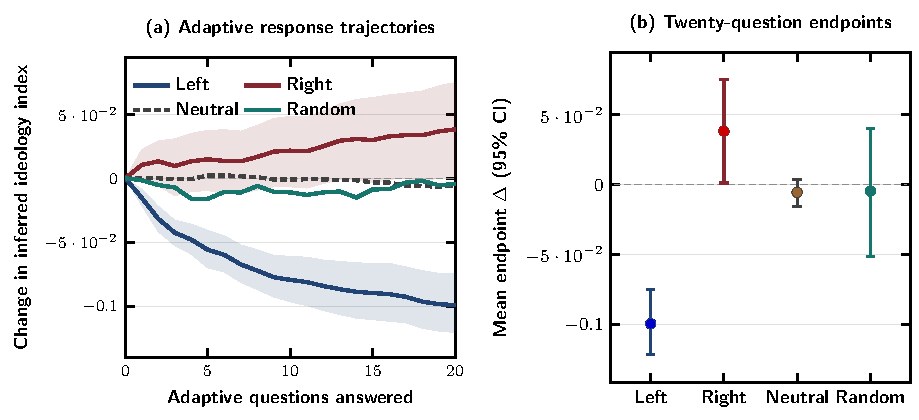
\includegraphics[width=\textwidth]{Figures/External/humanstudy}

\vspace{-10pt}
\caption{\textbf{Human study response trajectories and endpoints.}
(a) The mean change from baseline in the LSM-derived ideology coordinate as
adaptive questions are answered, with pointwise 95\% participant-bootstrap
confidence intervals shaded only for Left and Right. Partial sessions contribute
only through their last observed step. (b) Endpoint means and 95\% bootstrap
confidence intervals for all four policies, calculated from participants with
all 20 adaptive answers. Arm sample sizes are reported in
Table~\ref{tab:humanstudy-participants}.}
\label{fig:humanstudy-trajectory-endpoints}


\end{figure*}



\subsection{Interpretation}
The human results support the directional-steering hypothesis. At
question 20, Left moved the inferred ideology index by $-0.0783$
(95\% bootstrap CI $[-0.1130,-0.0195]$), and Right moved it by
$+0.0382$ (CI $[+0.0012,+0.0748]$). Neutral ($-0.0054$) and
Random ($-0.0045$) showed substantially smaller mean changes.
The Right arm included 11 participants with negative and six with
positive baseline indices; rightward mean movement therefore occurred
in a cohort spanning both sides of the initial ideology coordinate.

Together with the native simulations, these human-response results
demonstrate directional control over the \emph{inferred ideology
index} through adaptive question selection. Defining displacement
relative to each participant's own baseline allows this effect to
be evaluated across heterogeneous starting states.
